\documentclass[11pt]{article}

\usepackage[margin=1in]{geometry}
\usepackage{array}
\usepackage{booktabs}
\usepackage{longtable}
\usepackage{hyperref}
\usepackage{amsmath}
\usepackage{tikz}
\usetikzlibrary{arrows.meta,positioning}

\newcommand{\code}[1]{\texttt{\detokenize{#1}}}
\newcommand{\B}[1]{#1B}
\newcommand{\M}[1]{#1M}
\newcommand{\K}[1]{#1K}
\setlength{\parskip}{0.55em}
\setlength{\parindent}{0pt}
\sloppy

\title{Metis: A Transparent Small-Model Research Line from Single-H100 Training to Sparse Multi-Accelerator Pretraining}
\author{Giulianno Vollmer\\Lernex\\\texttt{giulianno@lernex.net}}
\date{May 24, 2026}

\begin{document}
\maketitle

\begin{abstract}
This technical report documents the Metis language-model line, an independent
research program focused on compact educational and reasoning-oriented language
models under constrained compute. Metis-1.3 and Metis-1.4 were developed as
single-H100-class release lines, producing public base, chat, and reasoning
checkpoints on Hugging Face. Metis-1.5 is the next step: a 1B-class sparse
decoder whose current manifest contains exactly 897,428,576 total parameters and
339,586,144 active parameters per token at depth one. The report details the
transition from a 201M-parameter Mamba2-attention hybrid, to a corrected
503.8M-parameter Mixture-of-Recursion (MoR) model, to a single-latent
mixture-of-experts (MoE) design with 32 routed experts, top-4 routing, one
shared expert, and an 8-way expert-parallel training target. We also describe
the Metis-1.5 curriculum: 50B tokens of base pretraining, 10B tokens of
continued pretraining, 1.2M chat SFT examples, 600K reasoning SFT examples,
400K reward-model preference pairs, and 300K DPO pairs. The central claim is not
state-of-the-art performance. The report argues that small-model research
should document not only final checkpoints, but also failed runs, hardware
constraints, and architecture accounting. Instead, the central claim is that
small-model research is more credible when architecture manifests, training
data plans, repaired failures, hardware constraints, and public model artifacts
are documented together.
\end{abstract}

\section{Introduction}

The Metis project began as a small local training stack and became a model line:
Metis-1.3, Metis-1.4, and the current Metis-1.5 architecture. Its target domain
is educational AI: models that can support tutoring, short-form reasoning,
writing help, and study workflows without assuming frontier-scale inference
budgets.

The project is also a compute-constrained architecture study. Each generation
asks a practical question: what can be learned when a small team keeps the
training path inspectable and treats hardware availability as a first-class
constraint? Metis-1.3 and Metis-1.4 were single-H100-class milestones. Metis-1.5
is explicitly beyond that comfort zone: it is a sparse, expert-parallel model
whose useful training path likely requires multi-accelerator capacity, such as
8xA100/8xH100 GPU nodes or AWS Trainium nodes.

This report has five goals:

\begin{enumerate}
  \item record the public Metis-1.3 and Metis-1.4 release line accurately;
  \item explain why Metis-1.5 is a 1B-class model even though the current
  manifest's exact total is 897.4M parameters;
  \item separate total parameters, active parameters, and parameter applications
  per token for sparse MoE accounting;
  \item document the exact Metis-1.5 training data plan; and
  \item state limitations plainly, especially where the project still needs
  clean benchmark results and full data-hygiene passes.
\end{enumerate}

\section{Design Goals}

Metis is optimized around four design goals.

\textbf{Small enough to iterate.} Metis is not a frontier-scale model family.
The project intentionally studies 0.2B to 1B-class models where architecture,
data, and training contracts can be inspected without massive institutional
compute.

\textbf{Useful for learning tasks.} The target behavior is not generic chatbot
imitation alone. The data plan emphasizes educational web text, reference
material, math/proof prose, scientific explanations, tutoring-like chat, and
short reasoning.

\textbf{Transparent research trail.} Model cards, manifests, training plans,
and failure notes are treated as research artifacts. A corrected model release
should say what it corrected.

\textbf{Hardware-aware architecture.} The model shape must map to available
accelerators. Metis-1.5 is sparse because the project needs more capacity per
token than dense single-GPU scaling provides, but sparse MoE only matters if the
dispatch and expert-parallel path can run efficiently on real hardware.

\section{Related Work}

Metis builds on standard decoder-only language modeling and transformer
components \cite{vaswani2017attention}. Metis-1.3 uses a Mamba2-attention hybrid
backbone, drawing from selective state-space models and structured state-space
duality \cite{gu2023mamba,dao2024mamba2}. Unlike a pure Mamba or Mamba2 model,
Metis-1.3 keeps attention layers in the stack so the project can study state
space sequence modeling without abandoning transformer-compatible tooling.
Metis-1.4 explores recursion over a shared transformer stack, while Metis-1.5
moves toward conditional computation through mixture-of-experts layers. The MoE
direction follows the broad lineage of sparsely gated expert layers, GShard,
Switch Transformer, and shared/routed expert specialization work
\cite{shazeer2017outrageously,lepikhin2020gshard,fedus2021switch,dai2024deepseekmoe}.

Metis is closest in scale and spirit to recent open small-model efforts such as
TinyLlama and SmolLM2, which show that careful data mixtures and long training
can make sub-2B models useful research artifacts rather than toys
\cite{zhang2024tinyllama,allal2025smollm2}. Metis differs by foregrounding a
multi-generation engineering record: the paper covers a 201M hybrid model, a
corrected 503.8M recursive model, and an untrained 1B-class sparse design rather
than reporting only a final trained checkpoint.

The project also takes inspiration from open model reports such as Pythia and
OLMo, which release checkpoints, code, data, or training details to make model
development scientifically inspectable \cite{biderman2023pythia,groeneveld2024olmo}.
Metis applies that norm at a smaller scale, including negative evidence:
quarantined artifacts, corrected label alignment, hardware ceilings, and
architecture accounting are part of the research record.

The project does not claim to invent these components. The contribution here is
the concrete model-development record: how they are combined, measured, revised,
and constrained under a small-model educational research program.

\section{Metis-1.3: 201M Mamba2-Attention Hybrid}

Metis-1.3 is the first stable public reference point in the current line. The
base model card describes a 201,490,560 parameter English-first decoder model
with a hybrid Mamba2 plus attention backbone \cite{metis13base}. Its key
architecture choices are:

\begin{itemize}
  \item 28 decoder blocks;
  \item 21 Mamba2 blocks and seven attention blocks;
  \item attention at layers 3, 7, 11, 15, 19, 23, and 27;
  \item grouped-query attention with 18 query heads and 6 key-value heads;
  \item 8192-token vocabulary;
  \item 4096-token context;
  \item tied embeddings and RMSNorm;
  \item BF16 release weights.
\end{itemize}

The public Metis-1.3 release includes base, chat, and think variants. The base
checkpoint is the raw pretrained model; the chat checkpoint adds supervised
fine-tuning for general instruction-following and conversation; the think
checkpoint adds a reasoning-focused SFT stage \cite{metis13base,metis13chat,metis13think}.

Metis-1.3 served two roles. First, it showed that the project could carry a
custom architecture from data preparation through release packaging. Second, it
created a concrete comparison target for later models: Metis-1.4 increased dense
capacity and tested recursion, while Metis-1.5 changes the feed-forward path to
sparse latent experts.

\section{Metis-1.4: Corrected 503.8M MoR Release}

Metis-1.4 is a compact 0.5B-class MoR-style model. The current public base card
states that the upload replaces an earlier experimental artifact with a
corrected base export from the repaired pipeline \cite{metis14base}. The current
Metis-1.4 release line includes base, chat, and think checkpoints
\cite{metis14base,metis14chat,metis14think}.

The corrected base model has:

\begin{itemize}
  \item approximately 503.8M parameters;
  \item 1024-token context;
  \item 16,384-token vocabulary;
  \item 1536 hidden width;
  \item 19 shared layers;
  \item grouped-query attention with 24 query heads and 8 key-value heads;
  \item SwiGLU feed-forward layers;
  \item RMSNorm and RoPE;
  \item BF16 exported weights after H100-oriented training.
\end{itemize}

The training story has two base stages. First, static dense pretraining trains
the shared transformer stack on the hot path. Second, static sequence-level MoR
continued pretraining reintroduces recursion with fixed-shape sequence groups.
That choice preserves static-shape efficiency while giving the model its first
recursion training signal.

An earlier Metis-1.4 artifact exposed a serious label-alignment bug: data
batches had been pre-shifted before entering a model loss that already performed
the next-token shift. That produced an accidental two-token-ahead objective. The
important point for this report is not that Metis-1.4 remains invalid; it does
not. The public base card now marks the current upload as the corrected base
export. The lesson retained for Metis-1.5 is that input/label alignment must be
tested as a training contract, not inferred from plausible loss curves.

\section{Metis-1.5: 1B-Class Single-Latent Sparse MoE}

\subsection{Exact Size and Why We Call It 1B-Class}

The current Metis-1.5 manifest reports exactly 897,428,576 total parameters,
339,586,144 active parameters at depth one, and 289,254,496 active transformer
parameters. It is therefore slightly below one billion parameters in the exact
current single-latent reset, but it remains a 1B-class model in planning,
memory, optimizer-state, and artifact terms. Earlier Metis-1.5 multi-head
LatentMoE drafts were above 1B total parameters; the current reset deliberately
trades some total parameters for a cleaner active-compute budget.

\begin{table}[h]
\centering
\begin{tabular}{ll}
\toprule
Field & Current manifest value \\
\midrule
Architecture & single-latent MoE decoder \\
Total parameters & 897,428,576 \\
Active parameters per token & 339,586,144 \\
Active transformer parameters & 289,254,496 \\
Layers & 19 \\
Hidden width & 1536 \\
Context length & 1024 \\
Vocabulary & 32,768 \\
Attention & 24 Q heads, 8 KV heads, head dim 64 \\
Experts & 32 routed, 1 shared \\
Routing & top-4 over one 512d latent route per token \\
Expert hidden width & 1024 \\
Default training dtype & BF16 \\
\bottomrule
\end{tabular}
\caption{Metis-1.5 current single-latent manifest summary.}
\label{tab:metis15_manifest}
\end{table}

\subsection{Routing Contract}

Metis-1.5 routes each token once. The hidden state starts at 1536 dimensions,
is projected to a 512-dimensional latent vector, is scored against 32 routed
experts, and activates the top four experts. Routed expert computation happens
in latent space. The result is projected back to the full hidden width and is
combined with a full-dimensional shared expert that remains active for every
token.

This reset is important. An earlier multi-head design routed four feature heads
independently, yielding 16 routed expert applications per token per layer. The
single-latent reset reduces that routing fan-out to four expert applications per
token per layer. That makes the model cheaper, easier to audit, and more
realistic to train before specialized MoE kernels are mature.

\begin{figure}[h]
\centering
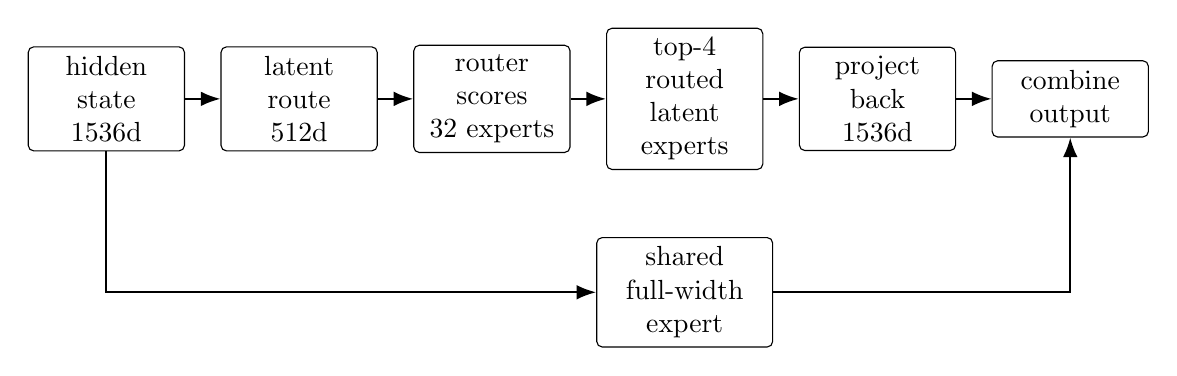
\begin{tikzpicture}[
  node distance=0.85cm and 0.45cm,
  box/.style={draw, rounded corners=2pt, align=center, minimum height=0.8cm, text width=1.75cm},
  smallbox/.style={draw, rounded corners=2pt, align=center, minimum height=0.7cm, text width=2.0cm},
  arrow/.style={-{Latex[length=2.5mm]}, thick}
]
\node[box] (hidden) {hidden state\\1536d};
\node[box, right=of hidden] (latent) {latent route\\512d};
\node[box, right=of latent] (router) {router scores\\32 experts};
\node[box, right=of router] (experts) {top-4 routed\\latent experts};
\node[box, right=of experts] (project) {project back\\1536d};
\node[box, right=of project] (combine) {combine\\output};
\node[smallbox, below=of experts] (shared) {shared full-width\\expert};
\draw[arrow] (hidden) -- (latent);
\draw[arrow] (latent) -- (router);
\draw[arrow] (router) -- (experts);
\draw[arrow] (experts) -- (project);
\draw[arrow] (project) -- (combine);
\draw[arrow] (hidden.south) |- (shared.west);
\draw[arrow] (shared.east) -| (combine.south);
\end{tikzpicture}
\caption{Metis-1.5 single-latent sparse MoE routing contract. Each token is
projected once into a 512d latent route, activates four of 32 routed experts,
and combines the projected routed result with a shared full-width expert.}
\label{fig:metis15_routing}
\end{figure}

\subsection{Compute Audit}

For sparse models, total parameters are not enough. Metis-1.5 therefore tracks
rough parameter applications per token:

\begin{itemize}
  \item embedding parameters: 50,331,648;
  \item attention applications per layer: 6,291,456;
  \item routed expert applications per layer: 4,194,304;
  \item shared expert applications per layer: 3,145,728;
  \item latent projection applications per layer: 1,572,864;
  \item router projection and matching applications per layer: 16,416;
  \item rough total parameter applications per token: 339,526,240;
  \item estimated training FLOPs per token: 2,037,157,440.
\end{itemize}

The launch gate for the current H100 path is a rough total of at most 450M
parameter applications per token. This is deliberately stricter than simply
asking whether the model fits in memory.

\section{Hardware Path}

Metis-1.3 and Metis-1.4 were single-H100-class milestones. Metis-1.4's H100
training stack used Hopper-oriented components such as FlashAttention-3,
Transformer Engine, FP8 training, and fused loss kernels. Dense Metis-1.4
throughput probes reached the 146K--170K token/s range depending on image and
kernel stack.

Metis-1.5 has a different bottleneck. On a single H100, stable BF16
\code{torch_grouped_safe} runs reached roughly 30.7K--31.1K token/s at batch 8
and context 1024. That is enough to prove the model path is alive, but not
enough for the full 60B-token base-plus-CPT plan. The limiting factor is not
only raw H100 compute. It is sparse MoE dispatch, grouped GEMM stability,
optimizer state, and launch overhead.

The near-term multi-accelerator targets are:

\begin{itemize}
  \item 8xA100 80GB as the conservative BF16 expert-parallel baseline;
  \item 8xH100 if quota and capacity are available;
  \item AWS Trainium as a credit-backed alternative if Neuron compilation can
  support the bounded dynamic-control-flow requirements.
\end{itemize}

The 8xA100 plan shards the 32 routed experts across eight ranks, so each rank
owns four routed experts per layer. Router, attention, latent projections,
shared experts, embeddings, final norm, and LM head remain replicated and
gradient-synchronized. Routed expert parameters remain rank-local.

For Trainium, the practical target is a 16-chip Trn1n node shape with 128 vCPUs,
512 GiB instance memory, 512 GB accelerator memory, 8 TB local NVMe, and 1600
Gbps networking \cite{aws-trn1}. Trainium is attractive because startup credits
may be easier to apply than scarce GPU capacity, but it is not a drop-in
assumption. Dynamic MoR and sparse routing need to be compiled as bounded static
loops with masks or otherwise mapped into Neuron-compatible shapes.

\section{Metis-1.5 Training Curriculum}

Metis-1.5 separates training into five stages:

\begin{enumerate}
  \item base pretraining: 50B tokens;
  \item continued pretraining/midtraining: 10B tokens;
  \item chat SFT: 1.2M examples;
  \item reasoning SFT: 600K examples;
  \item preference optimization: 400K reward-model pairs and 300K DPO pairs.
\end{enumerate}

The release plan is base plus think. The chat stage is an internal bridge into
the think checkpoint rather than a separate Metis-1.5 public target.

\subsection{Base Pretraining: 50B Tokens}

The base pretraining mix is intentionally broad but capped. It uses high-quality
web text for language coverage, reference sources for factual grounding,
academic and math material for reasoning, books for long-form coherence,
StackExchange-style explanations for answer structure, and a capped synthetic
educational slice. Table \ref{tab:pretrain_buckets} gives the bucket-level plan;
Appendix \ref{app:pretrain_sources} gives the source-level allocation.

\begin{table}[h]
\centering
\begin{tabular}{p{0.42\linewidth}r r}
\toprule
Bucket & Tokens & Share \\
\midrule
High-quality web, DCLM-style & 12B & 24\% \\
High-quality web, FineWeb-style & 9B & 18\% \\
Nemotron/newer quality web & 5B & 10\% \\
Reference and encyclopedic & 3B & 6\% \\
Academic STEM and science & 5B & 10\% \\
Math, proof, symbolic & 6B & 12\% \\
Open textbooks and educational reference & 3B & 6\% \\
Long-form books & 2B & 4\% \\
Knowledge QA and explanations & 2B & 4\% \\
Synthetic educational prose & 2B & 4\% \\
Reserve balancing pool & 1B & 2\% \\
\bottomrule
\end{tabular}
\caption{Metis-1.5 base pretraining bucket plan.}
\label{tab:pretrain_buckets}
\end{table}

\subsection{Continued Pretraining: 10B Tokens}

Continued pretraining concentrates the model on STEM, math/proof documents,
problem-solution prose, reference answers, technical PDFs, and science
instruction/literature text while retaining general replay. The purpose is to
move the model toward educational reasoning without destroying general language
behavior.

\begin{table}[h]
\centering
\begin{tabular}{p{0.48\linewidth}r r}
\toprule
Bucket & Tokens & Share \\
\midrule
High-quality general replay & 1.2B & 12\% \\
Academic STEM & 2.0B & 20\% \\
Math/proof documents & 2.0B & 20\% \\
Verifiable math problem-solution prose & 1.2B & 12\% \\
Reference/wiki/StackExchange & 1.2B & 12\% \\
FinePDFs technical OCR & 0.8B & 8\% \\
Science instruction/literature text & 0.6B & 6\% \\
Long-form book replay & 0.5B & 5\% \\
Hard general decontaminated examples & 0.5B & 5\% \\
\bottomrule
\end{tabular}
\caption{Metis-1.5 continued-pretraining bucket plan.}
\label{tab:cpt_buckets}
\end{table}

\subsection{Post-Training}

Chat SFT emphasizes useful assistant behavior without forcing long hidden
reasoning traces. Reasoning SFT then adds compact math, proof, science, and
general multistep reasoning. Preference optimization is planned as reward-model
training followed by DPO, with on-policy Metis-generated negatives included
after chat and think checkpoints exist.

\begin{table}[h]
\centering
\begin{tabular}{p{0.45\linewidth}r r}
\toprule
Stage or bucket & Target & Share \\
\midrule
Chat SFT total & 1.2M examples & 100\% \\
General instruction behavior & 300K & 25.0\% \\
Everyday chat/simple help & 210K & 17.5\% \\
Writing/summarization/rewriting & 140K & 11.7\% \\
Format following/constraints & 130K & 10.8\% \\
Knowledge/reference answers & 130K & 10.8\% \\
Science instruction & 90K & 7.5\% \\
Math light instruction & 80K & 6.7\% \\
Safety/refusal/harmlessness & 60K & 5.0\% \\
Legacy OpenHermes capped & 60K & 5.0\% \\
\bottomrule
\end{tabular}
\caption{Metis-1.5 chat SFT plan.}
\label{tab:chat_sft}
\end{table}

\begin{table}[h]
\centering
\begin{tabular}{p{0.45\linewidth}r r}
\toprule
Reasoning bucket & Examples & Share \\
\midrule
Math reasoning, medium/hard & 170K & 28.3\% \\
Hard math/olympiad/competition & 120K & 20.0\% \\
Proof/symbolic/formal-ish & 70K & 11.7\% \\
Science reasoning & 90K & 15.0\% \\
General multistep reasoning & 100K & 16.7\% \\
Tiny hard curated & 25K & 4.2\% \\
Simple arithmetic/GSM-style & 25K & 4.2\% \\
\bottomrule
\end{tabular}
\caption{Metis-1.5 reasoning SFT plan.}
\label{tab:reason_sft}
\end{table}

\begin{table}[h]
\centering
\begin{tabular}{p{0.48\linewidth}r r}
\toprule
Preference bucket & Reward pairs & DPO pairs \\
\midrule
HelpSteer3 filtered English non-code & 48K & 36K \\
Skywork Reward Preference & 72K & 54K \\
UltraFeedback cleaned & 48K & 36K \\
Tulu/OLMo preference mixes & 60K & 45K \\
Nectar filtered capped & 40K & 30K \\
Math/science correctness preferences & 40K & 30K \\
Safety/helpfulness pairs & 20K & 15K \\
On-policy Metis pairs & 72K & 54K \\
\bottomrule
\end{tabular}
\caption{Metis-1.5 preference-optimization plan.}
\label{tab:preference}
\end{table}

\section{Data Hygiene}

The Metis-1.5 data manifests are bucketed and validated. The current validation
script reports no structural errors across base pretraining, continued
pretraining, chat SFT, reasoning SFT, and preference optimization. It confirms,
among other things, 11 base-pretraining buckets, 9 continued-pretraining buckets,
9 chat buckets, 7 reasoning buckets, and preference targets of 400K reward pairs
and 300K DPO pairs.

That validation is necessary but not sufficient. Full serious training still
requires stronger English language identification, global near-deduplication,
code-ratio filtering, benchmark contamination checks, and bucket-local fallback
audits. The paper therefore treats the data plan as a training design and not as
evidence of completed decontaminated pretraining.

\section{Limitations}

Metis is early research. The report should not be read as evidence that the
Metis-1.5 architecture improves downstream accuracy until controlled training
and evaluation are complete. The main limitations are:

\begin{itemize}
  \item Metis-1.5 does not yet have final benchmark results in this report.
  \item The 60B-token plan is validated structurally, but the full filtering and
  decontamination pipeline still has to be completed before a major paid run.
  \item Single-H100 Metis-1.5 runs are useful for stability and profiling, but
  they are not the intended full-training path.
  \item Trainium support remains a compatibility question, especially around
  bounded dynamic MoR and sparse routing under Neuron compilation.
  \item Metis-1.3 and Metis-1.4 are small models and should not be treated as
  reliable production assistants.
\end{itemize}

\section{Conclusion}

Metis is a small-model research line built around transparent iteration. The
public Metis-1.3 and corrected Metis-1.4 releases show the single-H100-class
path. Metis-1.5 shows the next pressure point: a 1B-class sparse architecture
whose useful training path depends on multi-accelerator expert parallelism and
stronger data hygiene. The value of the project is not only in its checkpoints,
but in the paper trail around them: architecture manifests, source-level data
plans, corrected failures, hardware constraints, and public model cards.

\appendix

\section{Base Pretraining Source Allocation}
\label{app:pretrain_sources}

\footnotesize
\begin{longtable}{p{0.22\linewidth}p{0.43\linewidth}r p{0.18\linewidth}}
\toprule
Bucket & Source & Tokens & Role \\
\midrule
\endhead
high-quality web DCLM & \code{mlfoundations/dclm-baseline-1.0} & 7.0B & model-filtered English web \\
high-quality web DCLM & \code{HuggingFaceTB/dclm-edu} & 5.0B & educational web \\
high-quality web FineWeb & \code{HuggingFaceFW/fineweb-edu} & 5.0B & educational web breadth \\
high-quality web FineWeb & \code{epfml/FineWeb-HQ} & 4.0B & high-quality web \\
Nemotron/newer web & \code{EssentialAI/essential-web-v1.0} & 2.0B & newer curated web \\
Nemotron/newer web & \code{LLM360/TxT360} & 1.25B & English common crawl slice \\
Nemotron/newer web & \code{Zyphra/Zyda-2} & 1.25B & novelty-heavy web \\
Nemotron/newer web & \code{openbmb/Ultra-FineWeb} & 0.5B & recent capped web \\
reference & \code{HuggingFaceFW/finewiki} & 2.4B & structured reference \\
reference & \code{common-pile/wikimedia_filtered} & 0.6B & filtered Wikimedia \\
academic STEM & \code{allenai/peS2o} & 2.5B & papers and STEM prose \\
academic STEM & \code{EleutherAI/proof-pile-2} & 1.35B & arXiv/science prose \\
academic STEM & \code{common-pile/pubmed_filtered} & 0.5B & biomedical literacy cap \\
academic STEM & \code{HuggingFaceFW/finepdfs} & 0.615B & OCR technical PDFs \\
academic STEM & \code{crumb/openstax-text} & 0.035B & textbooks \\
math/proof & \code{nvidia/Nemotron-CC-Math-v1} & 2.8B & math web \\
math/proof & \code{HuggingFaceTB/finemath} & 1.2B & high-score math \\
math/proof & \code{open-web-math/open-web-math} & 0.8B & equation-rich web \\
math/proof & \code{EleutherAI/proof-pile-2} & 0.7B & proof prose \\
math/proof & \code{LLM360/MegaMath} & 0.5B & web proof/math \\
textbooks/reference & \code{crumb/openstax-text} & 0.035B & clean textbooks \\
textbooks/reference & \code{PleIAs/common_corpus} & 1.765B & educational reference \\
textbooks/reference & \code{common-pile/comma_v0.1_training_dataset} & 1.2B & educational filtered \\
long-form books & \code{deepmind/pg19} & 0.8B & long-form coherence \\
long-form books & \code{common-pile/project_gutenberg_filtered} & 0.7B & filtered books \\
long-form books & \code{PleIAs/common_corpus} & 0.5B & Wikisource/books \\
QA/explanations & \code{common-pile/stackexchange_filtered} & 1.2B & accepted-answer style \\
QA/explanations & \code{bigscience-data/roots_en_no_code_stackexchange} & 0.5B & non-code Q/A \\
QA/explanations & \code{HuggingFaceFW/fineweb-edu} & 0.3B & explainer-mined web \\
synthetic educational & \code{HuggingFaceTB/smollm-corpus/cosmopedia-v2} & 1.5B & capped synthetic textbooks \\
synthetic educational & \code{HuggingFaceTB/smollm-corpus/cosmopedia-v2} & 0.5B & selected explainers \\
reserve & \code{allenai/peS2o} & 0.4B & underrepresented STEM \\
reserve & \code{HuggingFaceFW/finewiki} & 0.3B & underrepresented reference \\
reserve & \code{nvidia/Nemotron-CC-Math-v1} & 0.3B & underrepresented math \\
\bottomrule
\end{longtable}
\normalsize

\section{Continued-Pretraining Source Allocation}

\footnotesize
\begin{longtable}{p{0.23\linewidth}p{0.43\linewidth}r p{0.17\linewidth}}
\toprule
Bucket & Source & Tokens & Role \\
\midrule
\endhead
general replay & \code{mlfoundations/dclm-baseline-1.0} & 0.6B & preserve general English \\
general replay & \code{HuggingFaceFW/fineweb-edu} & 0.6B & preserve education web \\
academic STEM & \code{allenai/peS2o} & 0.93B & STEM papers \\
academic STEM & \code{EleutherAI/proof-pile-2} & 0.7B & arXiv math/physics/CS \\
academic STEM & \code{crumb/openstax-text} & 0.015B & textbooks \\
academic STEM & \code{common-pile/pubmed_filtered} & 0.2B & biomedical cap \\
academic STEM & \code{HuggingFaceFW/finepdfs} & 0.155B & academic PDFs \\
math/proof docs & \code{nvidia/Nemotron-CC-Math-v1} & 0.8B & math web \\
math/proof docs & \code{EleutherAI/proof-pile-2} & 0.5B & proof documents \\
math/proof docs & \code{HuggingFaceTB/finemath} & 0.3B & math quality slice \\
math/proof docs & \code{open-web-math/open-web-math} & 0.3B & equation-rich web \\
math/proof docs & \code{LLM360/MegaMath} & 0.1B & web proof/math \\
problem-solution & \code{open-r1/OpenR1-Math-220k} & 0.4B & verified math prose \\
problem-solution & \code{AI-MO/NuminaMath-CoT} & 0.3B & solution prose \\
problem-solution & \code{nvidia/OpenMathInstruct-2} & 0.3B & verified sample \\
problem-solution & \code{AI-MO/NuminaMath-TIR} & 0.2B & plain text TIR \\
reference/Q\&A & \code{HuggingFaceFW/finewiki} & 0.4B & reference \\
reference/Q\&A & \code{common-pile/stackexchange_filtered} & 0.4B & explanations \\
reference/Q\&A & \code{PleIAs/common_corpus} & 0.4B & education/reference \\
technical OCR & \code{HuggingFaceFW/finepdfs} & 0.8B & long technical PDFs \\
science text & \code{allenai/SciRIFF} & 0.3B & science tasks as text \\
science text & \code{zd21/SciInstruct} & 0.3B & science instruction prose \\
book replay & \code{deepmind/pg19} & 0.25B & long-form retention \\
book replay & \code{common-pile/project_gutenberg_filtered} & 0.25B & filtered books \\
hard general & \code{HuggingFaceTB/dclm-edu} & 0.25B & hard education web \\
hard general & \code{HuggingFaceFW/fineweb-edu} & 0.25B & hard education web \\
\bottomrule
\end{longtable}
\normalsize

\section{Primary References}

\begin{thebibliography}{99}

\bibitem{vaswani2017attention}
Ashish Vaswani et al.
\newblock Attention Is All You Need.
\newblock \emph{arXiv:1706.03762}, 2017.

\bibitem{gu2023mamba}
Albert Gu and Tri Dao.
\newblock Mamba: Linear-Time Sequence Modeling with Selective State Spaces.
\newblock \emph{arXiv:2312.00752}, 2023.

\bibitem{dao2024mamba2}
Tri Dao and Albert Gu.
\newblock Transformers are SSMs: Generalized Models and Efficient Algorithms Through Structured State Space Duality.
\newblock \emph{arXiv:2405.21060}, 2024.

\bibitem{shazeer2017outrageously}
Noam Shazeer et al.
\newblock Outrageously Large Neural Networks: The Sparsely-Gated Mixture-of-Experts Layer.
\newblock \emph{arXiv:1701.06538}, 2017.

\bibitem{lepikhin2020gshard}
Dmitry Lepikhin et al.
\newblock GShard: Scaling Giant Models with Conditional Computation and Automatic Sharding.
\newblock \emph{arXiv:2006.16668}, 2020.

\bibitem{fedus2021switch}
William Fedus, Barret Zoph, and Noam Shazeer.
\newblock Switch Transformers: Scaling to Trillion Parameter Models with Simple and Efficient Sparsity.
\newblock \emph{arXiv:2101.03961}, 2021.

\bibitem{dai2024deepseekmoe}
Damai Dai et al.
\newblock DeepSeekMoE: Towards Ultimate Expert Specialization in Mixture-of-Experts Language Models.
\newblock \emph{arXiv:2401.06066}, 2024.

\bibitem{zhang2024tinyllama}
Peiyuan Zhang, Guangtao Zeng, Tianduo Wang, and Wei Lu.
\newblock TinyLlama: An Open-Source Small Language Model.
\newblock \emph{arXiv:2401.02385}, 2024.

\bibitem{allal2025smollm2}
Loubna Ben Allal et al.
\newblock SmolLM2: When Smol Goes Big -- Data-Centric Training of a Small Language Model.
\newblock \emph{arXiv:2502.02737}, 2025.

\bibitem{biderman2023pythia}
Stella Biderman et al.
\newblock Pythia: A Suite for Analyzing Large Language Models Across Training and Scaling.
\newblock \emph{arXiv:2304.01373}, 2023.

\bibitem{groeneveld2024olmo}
Dirk Groeneveld et al.
\newblock OLMo: Accelerating the Science of Language Models.
\newblock \emph{arXiv:2402.00838}, 2024.

\bibitem{metis13base}
Giulianno Vollmer.
\newblock Metis-1.3 Base.
\newblock Hugging Face model card, \url{https://huggingface.co/Lernex/Metis-1.3-base}, 2026.

\bibitem{metis13chat}
Giulianno Vollmer.
\newblock Metis-1.3 Chat.
\newblock Hugging Face model card, \url{https://huggingface.co/Lernex/Metis-1.3-chat}, 2026.

\bibitem{metis13think}
Giulianno Vollmer.
\newblock Metis-1.3 Think.
\newblock Hugging Face model card, \url{https://huggingface.co/Lernex/Metis-1.3-think}, 2026.

\bibitem{metis14base}
Giulianno Vollmer.
\newblock Metis-1.4 Base.
\newblock Hugging Face model card, \url{https://huggingface.co/Lernex/Metis-1.4-base}, 2026.

\bibitem{metis14chat}
Giulianno Vollmer.
\newblock Metis-1.4 Chat.
\newblock Hugging Face model card, \url{https://huggingface.co/Lernex/Metis-1.4-chat}, 2026.

\bibitem{metis14think}
Giulianno Vollmer.
\newblock Metis-1.4 Think.
\newblock Hugging Face model card, \url{https://huggingface.co/Lernex/Metis-1.4-think}, 2026.

\bibitem{aws-trn1}
Amazon Web Services.
\newblock Amazon EC2 Trn1 Instances.
\newblock \url{https://aws.amazon.com/ec2/instance-types/trn1/}, accessed May 24, 2026.

\end{thebibliography}

\end{document}
